\FloatBarrier
\section{CUDA Experiments}

Section~\ref{sec:CUDAImpl} discusses the possibility of using CUDA to enable GPU-assisted execution of sorting networks, to speed up their computations through massive parallelism. This section shows the actual results of moving large parts of the program to the GPU, and examines how much of a speed gain is attainable both on old and new GPUs.

Programs were run on the machine described in Section 5.1, featuring a graphics card that is targeted at professional GPU-intensive applications, but is rather dated, and on a newer machine featuring a modern GPU targeted at computer gaming.

The newer machine has the following specifications:

\begin{description}
\item[CPU:] Intel i7-4810MQ, 2.8GHz, 6 MB Cache
\item[RAM:] 8GB
\item[GPU:] NVIDIA GeForce GTX 870M 
\item[Operating System:] Ubuntu 14.04 LTS
\end{description}

All CUDA implementations were separately compiled objects, and linked into the main program, to preserve sequential behaviour when CUDA is not in use. The CUDA objects were written in CUDA C++, and compiled with the following additional parameters, parameters separated by slashes varied between GPU architectures.

\begin{description}
\item[\texttt{-O3}] Use the highest optimization level
\item[\texttt{-arch=compute\_12 / -arch=compute\_30}] Optimize compilation for the specified architecture.
\item[\texttt{-code=sm\_12 / code=sm\_30}] Optimize code generation for the specified architecture.
\item[\texttt{-{}-maxregcount 16}] Use a maximum of 16 registers per thread, allowing full occupancy for all cards from CUDA 1.2 and up. 
\end{description}


\subsection{Improvements in Running Time}

Since we are now comparing different architectures, it makes little sense to consider hardware-specific metrics such as branch mispredictions and cache misses, so let us instead focus entirely on the running time, and what gains can be made by offloading parts of the program to the GPU.

Figure~\ref{fig:CUDAQuadro:time} and~\ref{fig:CUDAGTX:time} show the running time of the different algorithms when using CUDA on the different architectures.
There are three main things to notice in these, independent of the graphics cards. Firstly, Randomized Shellsort has a much better time handling cache misses when using the GPU, since we offload the random memory accesses to the GPU, and since the GPU has a much higher memory bandwith than the GPU, it seems to cope better with these access patterns.
Secondly, the other CUDA-assisted algorithms all seem to perform well, and even seem to have a running time that is close to $O(n \log n)$ in practice when they can use the GPU for massively parallel computations.
Finally, CUDA-based Bitonic Sort outperforms all other algorithms on the chart. This shows the power of migrating the entire algorithm to the GPU, and properly utilizing the memory manipulation options of the CUDA architecture.

\begin{figure}
\center
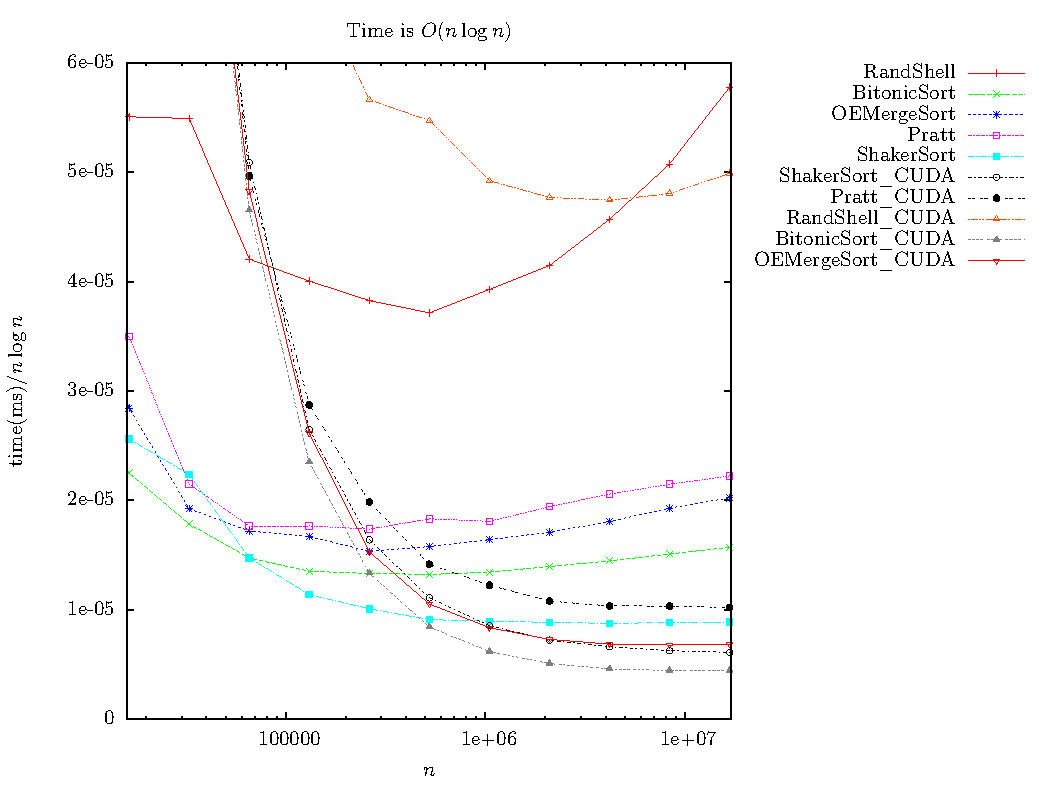
\includegraphics[width=\textwidth]{graphs/CUDA/nlogntime.pdf}
\caption{Time with and without CUDA, Quadro FX 880M}
\label{fig:CUDAQuadro:time}
\end{figure}


\begin{figure}
\center
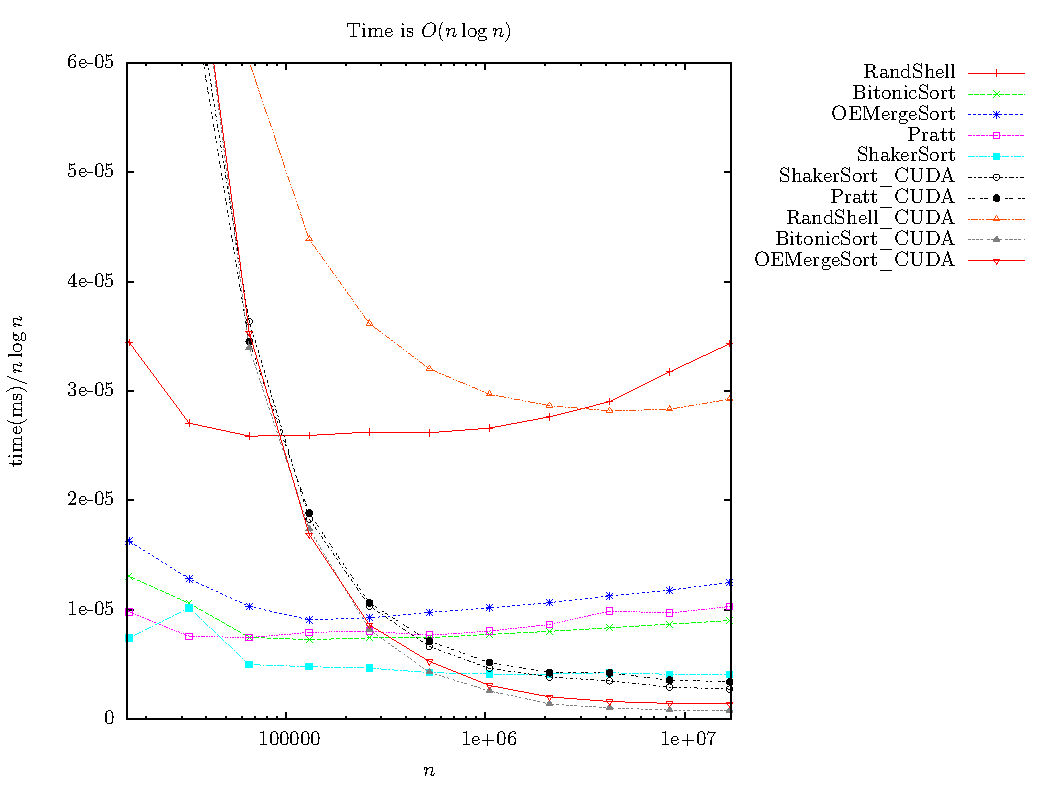
\includegraphics[width=\textwidth]{graphs/CUDAHueg/nlogntime.pdf}
\caption{Time with and without CUDA, GTX 870M}
\label{fig:CUDAGTX:time}
\end{figure}


In fact, let us further expand the view of the CUDA-enabled algorithms, Randomized Shellsort excluded.

Figure~\ref{fig:CUDAQuadro:cudatime} and~\ref{fig:CUDAGTX:cudatime} shows a view of a small selection of the included algorithms, with \texttt{std::sort}. The graphs are given the same scale on the y-axis, so the running times are directly comparable.

What we see here, is that the CUDA-assisted algorithms start out relatively slow, but provide excellent scalability as the input size increases, and in fact seem to be nearing an $O(n \log n)$ running time due to the massively parallel execution. This comes as a big surprise in the case of the algorithms that would normally be $\Theta(n \log^2 n)$, as the CUDA-implementations are supposed to have similar asymptotic running times. It is hard to explain exactly how the GPU achieves this, but most likely, the GPU scales well with a large amount of threads, and the additional logarithmic factor is getting overshadowed by the GPU scaling to larger input sizes.

Most impressive of all, are the running times presented in Figure~\ref{fig:CUDAGTX:cudatime}, where we see the CUDA-assisted sorting networks thoroughly outperform \texttt{std::sort}.

\begin{figure}
\center
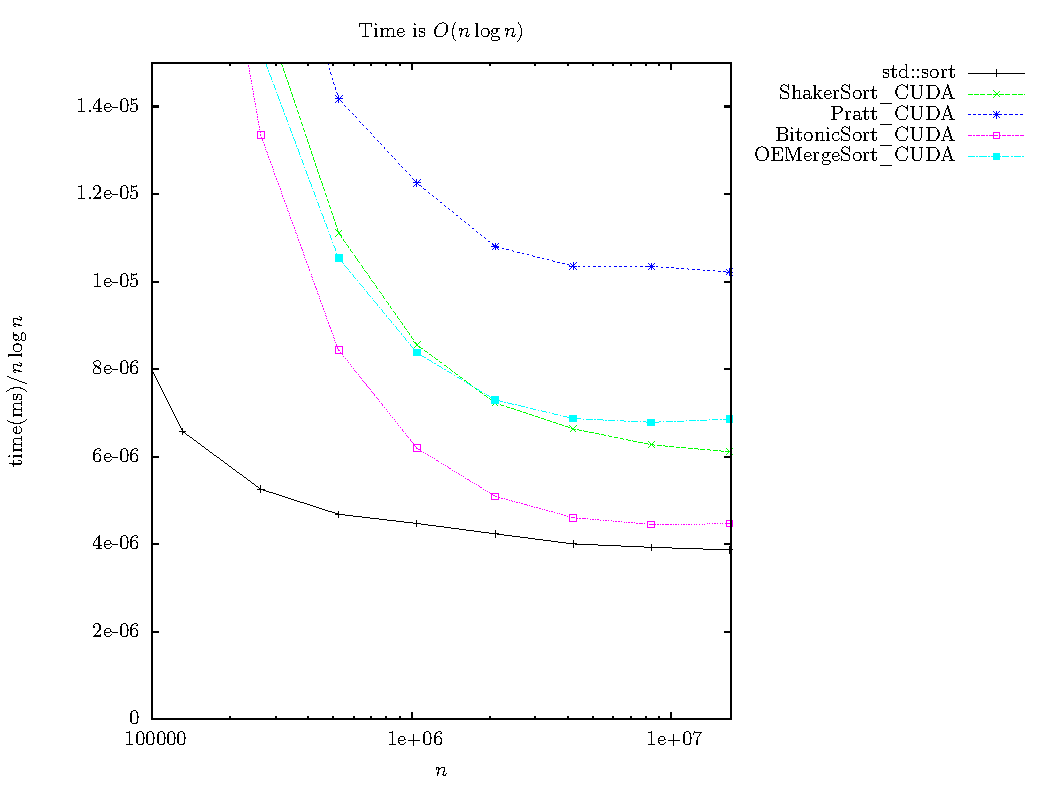
\includegraphics[width=\textwidth]{graphs/CUDA/cudatime.pdf}
\caption{Sectioned time with and without CUDA, Quadro FX 880M}
\label{fig:CUDAQuadro:cudatime}
\end{figure}

\begin{figure}
\center
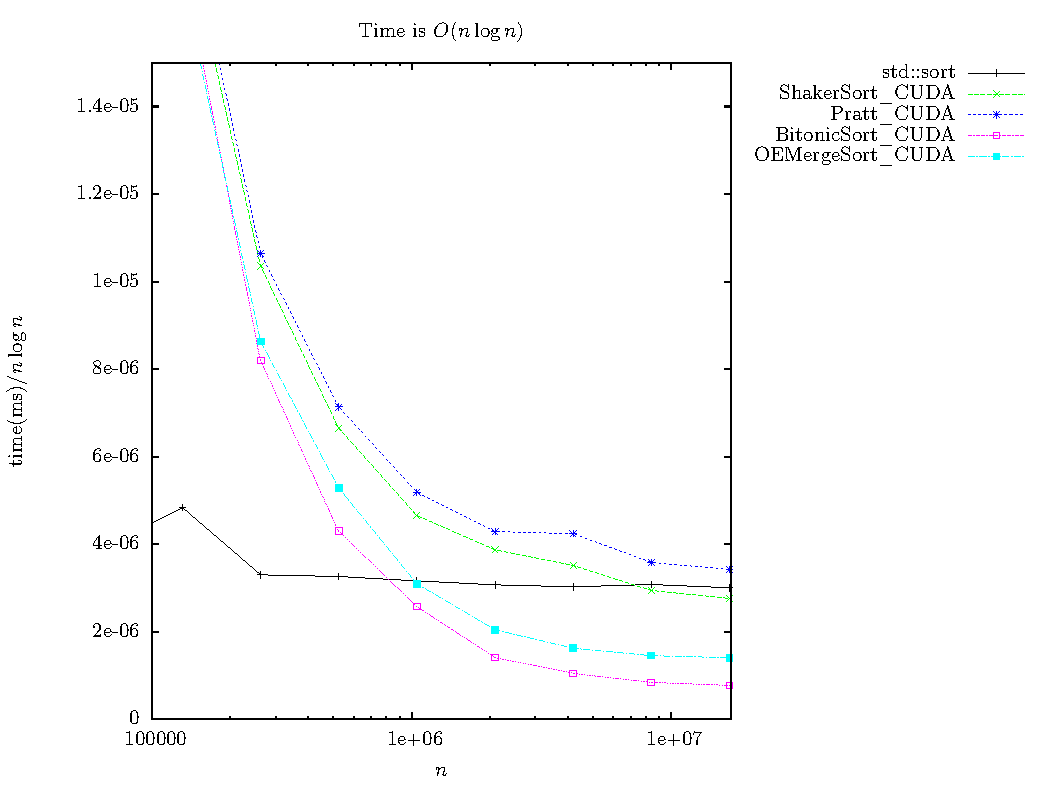
\includegraphics[width=\textwidth]{graphs/CUDAHueg/cudatime.pdf}
\caption{Sectioned time with and without CUDA, GTX 870M}
\label{fig:CUDAGTX:cudatime}
\end{figure}

Finally, let us consider how much the individual algorithms benefit from allowing CUDA-execution of certain sections. Figure~\ref{fig:CUDAQuadro:timediff} and~\ref{fig:CUDAGTX:timediff} shows the factor with which we can reduce the running times of the algorithms depending on the graphics card.

For Randomized Shellsort, we see a small but noticeable gain when input sizes grow, which can be explained by the work sharing between GPU and CPU. Note that the GPU-assisted verison of Randomized Shellsort does not seem to be impacted as heavily by the cache limit as as the seqeuntial one.

For the Shellsort variants, we see a respectable gain. This gain is caused by the adaptability of h-shakes on the GPU, as these exhibit both excellent parallelism, but also good memory access patterns. The Shellsort variants do however suffer from not having their entire execution moved to the GPU. Note that Pratt's Shellsort benefits more from GPU-acceleration than Shaker sort, which might be due to either having a larger amount of high-distance h-shakes, or simply being slightly slower on the CPU.

The last algorithms, Bitonic Sort and Odd-Even Mergsort shows massive gains from applying CUDA execution. This is due to being moved to the GPU in their entirety, and having excellent adaptability to parallelism. The newer graphics card show an exceptional performance gain compared to the specialized card from the older machine. Note that the slightly larger gain to Bitonic sort compared to Odd-Even Mergesort due to the utilization of thread-local memory.

\begin{figure}
\center
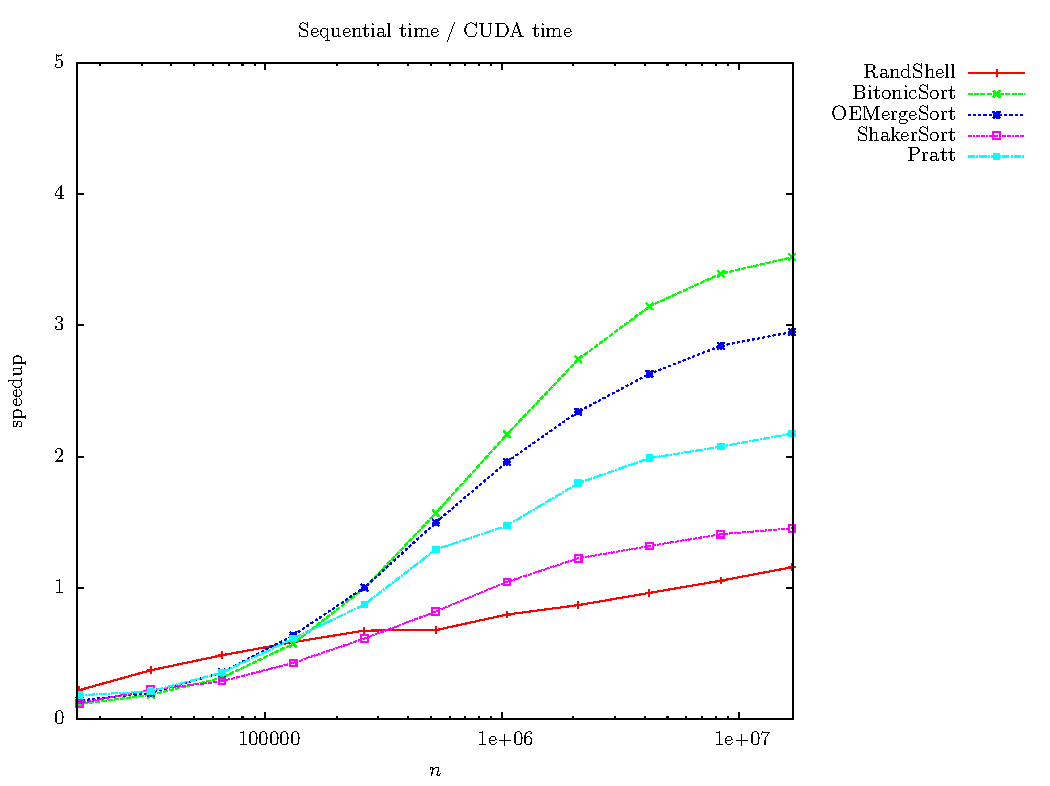
\includegraphics[width=\textwidth]{graphs/CUDA/timediff.pdf}
\caption{Time factor with and without CUDA, Quadro FX 880M}
\label{fig:CUDAQuadro:timediff}
\end{figure}

\begin{figure}
\center
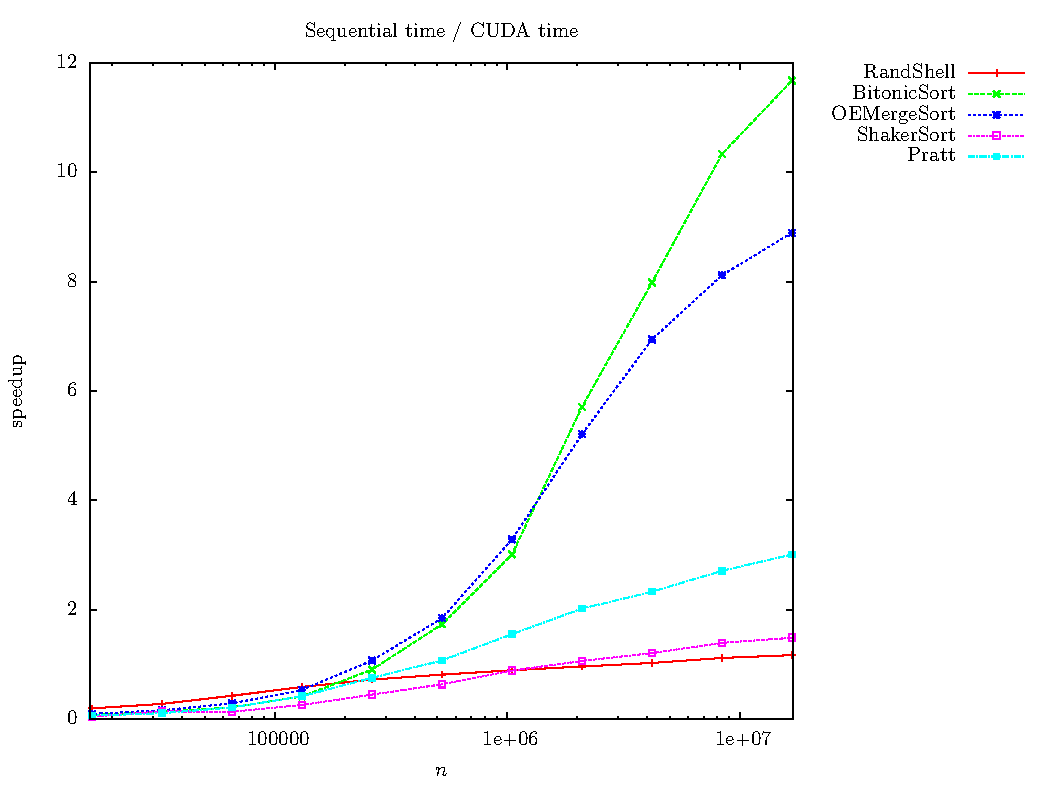
\includegraphics[width=\textwidth]{graphs/CUDAHueg/timediff.pdf}
\caption{Time factor with and without CUDA, GTX 870M}
\label{fig:CUDAGTX:timediff}
\end{figure}

\subsection{Experiment Conclusion}

The experiment showed that many of the algorithms benefit well from GPU-assisted execution, but the amount of speed-up gained varies widely between the different algorithms.

We've seen that with the $\Theta(n \log^2 n)$ algorithms, the GPU-parallelism seems the somehow make up for the additional logarithmic factor in execution time, and make these algorithms approach an $O(n \log n)$ running time in practise.

Especially the classic sorting networks of~\citeA{SNApplications} show a great suitability for GPU sorting, and even beats \texttt{std::sort} on modern hardware.